\documentclass{beamer}

\usepackage{amsmath}
\usepackage{amsfonts}
\usepackage{amssymb}
\usepackage[utf8]{inputenc}
\usepackage[spanish, mexico]{babel}

\usetheme{Warsaw}


\title{Presentación}
\author{Miguel A. Gomez}
\institute{Fundación Universitaria Konrad Lorenz}
\date{20-08-2019}

\begin{document}
	\begin{frame}
		\frametitle{Andrew John Wiles (Abril 11, 1963)}
		\framesubtitle{¿Quién?}
		\begin{columns}
			\column{0.5\textwidth}
			\begin{figure}
				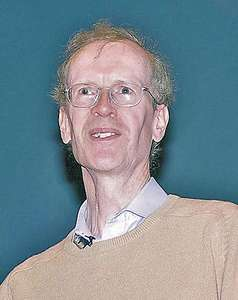
\includegraphics[width=0.9\linewidth]{andrew_wiles.jpg}
				\caption{Andrew Wiles.}
				\label{fig:andrew}
			\end{figure}
			
			\column{0.5\textwidth}
			Nacido en Cambridge Inglaterra, ha trabajado en un amplio número de de problemas en teoría de números, siendo su trabajo más destacado la demostración de la conjetura Shimura-Taniyama-weil que demuestra la conjetura de Fermat. Esta conjetura cautivó a Wiles desde muy pequeño al leer el libro \textit{El último teorema} de E.T. Bell, Ello lo motivó a convertirse en matemático.
		\end{columns}
	\end{frame}
	\begin{frame}
		\frametitle{Andrew John Wiles (Abril 11, 1963)}
		\framesubtitle{¿Porqué es importante?}
		\begin{itemize}
			\item En su publicación \textit{"Modular Elliptic Curves and Fermat’s Last Theorem"} (de 130 páginas), demostró uno de los problemas del milenio, uno de los teoremas en el que ni siquiera matemáticos como Gauss y Euler pudieron resolver con herramientas de su época.
			\item Su trabajo en esta prueba tiene implicaciones en otras ramas de la matemática que son actualmente objeto de estudio.
		\end{itemize}
		
	\end{frame}

\end{document}